\documentclass[]{article}
\usepackage{amsmath}
\usepackage{amssymb}
\usepackage{graphicx}
\usepackage{subcaption}
\usepackage{tabularx}
\usepackage{float}
\usepackage{hyperref}

\usepackage{chato-notes}

\newcolumntype{b}{X}
\newcolumntype{s}{>{\hsize=.5\hsize}X}

\newcommand{\commG}[1]{#1}
%\newcommand{\commG}[1]{}

\newcommand{\abs}[1]{\left\lvert#1\right\rvert}
%\newcommand{\normnoStar}[1]{\left\lVert#1\right\rVert}

\newcommand{\spc}{i}
\newcommand{\ospc}{j}
\newcommand{\site}{k}
\newcommand{\AssMat}{A}
\newcommand{\EffMat}{Q}
\newcommand{\ResMat}{P}
\newcommand{\BioCont}{C}
\newcommand{\BioEff}{z}
\newcommand{\abiov}{x}
\newcommand{\abdv}{y}
\newcommand{\abioM}{X}
\newcommand{\abdM}{Y}
\newcommand{\ssuit}{s}

\newcommand{\habs}{h}
\newcommand{\linkf}{f}

\DeclareMathOperator{\avg}{avg}
\DeclareMathOperator{\std}{std}

%opening
\title{Uncovering ecological associations by learning latent representations of species effects and responses from their co-distribution}
\author{Sara Si-moussi, Esther Galbrun, Mickael Hedde, Wilfried Thuiller}

\graphicspath{ {./images/} }
\begin{document}

\maketitle

\section{Background}
To understand the drivers of species distribution and their abundance
is an age-old question in biogeography (von Humboldt 1805). Niche
theory explains the geographical dynamics of species by a set of
properties and adaptive behaviors they exhibit that allows them to
thrive in specific conditions and decline in others (Chase and Leibold
2003, Peterson 2011).  At a macroscopic scale, the potential habitat
of a species is delimited by the ranges of abiotic variables, such as
climate and soil characteristics, that match the ecophysiological
requirements of the species. This potential niche is refered to as the
\emph{Grinnellian niche} (Grinnell 1917) or the \emph{fundamental
  niche} (Hutchinson 1957).  Habitat Suitability Models (HSM) and
Species Distribution Models (SDM) aim to infer this niche by
establishing statistical relationships between observed presences
(realized niche) and the environmental characteristics of the
corresponding locations (Hirzel 2008).

SDMs have proven useful to predict species ranges in response to
climate change, providing operational tools to conservation biologists
(Guisan and Thuiller 2005, Elith 2006). However, they predict multiple
species distributions separately, ignoring possible dependencies that
can restrict or extend species' ranges as compared to what is expected
when considering only abiotic factors.  Indeed, species may exclude
one another locally (\emph{competitive exclusion}, Gause 1934) or
differentiate each other's areas and resources (\emph{niche
  partitioning}, Schoner 1974). Conversely, some species facilitate
others by modifying the environment in a way that creates habitats or
enables access to resources for other species (\emph{engineering} and
\emph{facilitation}, Boucher 1982).  Although these interactions take
place at a local scale, some of them may restrict the range of the
species on a wider, macroscopic scale.  Thus, the inability to take
into account the presence or absence of other species is an important
source of underfitting for SDMs (Wisz 2013).

Over the last decade, several approaches have been proposed to infer
interspecific associations within the latter models by jointly
analyzing the co-distribution of multiple species. This led to the
development of Joint Species Distribution Models (JSDM) by Pollock et
al.\ (2014). The gist is that once we have accounted for abiotic
factors, the unexplained variance, typically captured by the residuals'
correlation matrix, is attributed to the effect of
species on one another. As they rely purely on correlation, JSDMs are
limited to inferring symmetric associations between species, such as
mutualism and competition. Asymmetric interactions, such as
commensalism, amensalism and predation, are therefore inherently out
of reach for these models. Lany et al.\ (2018) proposed a JSDM that
allows to capture asymmetric associations but it requires access to
longitudinal data.

\medskip Another research domain that is also concerned with inferring
associations from co-occurrence is natural language processing
(NLP). NLP modelers try to understand semantic associations between
words on the basis of the contexts they appear in. The context of a
word is the list of words surrounding it in a sentence. A state of art
method in this area is \texttt{word2vec} (Mikolov et al
2013). \texttt{word2vec} learns distributed representations for words
in the form of dense vectors called embeddings. The embedding of a
word captures information about other words it co-occurs with. The
probability of a word occurring in a particular sentence of a text
depends on the semantic compatibility of this word with other words
occurring in that sentence. Word embeddings, such as
\texttt{word2vec}, aim to learn multidimensional representations of
words that captures this contextual semantic compatibility. By
analogy, in community ecology, the probability of the presence of a
species in a given abiotically suitable site depends on its
compatibility with other species occuring at that site, i.e.\ other
species in the observed community.
Rudolph et al.\ (2016) introduced a generalization of word embeddings to
any type of data that follow an exponential family distribution,
including binary and ordinal data, called exponential family
embeddings.

Building on existing work, we propose a conditional
probabilistic model of species co-distributions that can be trained
jointly with any habitat suitability model on presence/absence or
count data to infer interspecific associations. We evaluate the
potential of the model to recover correct associations on empirically
observed as well as simulated communities.

\section{Material and Methods}
Three main factors determine the presence and abundance of a species
in a given location.  First, the location must be accessible from the
biogeographic origins of the species. This relates to the dispersal
capacity of the species and the presence of migration corridors or
barriers.  Second, the species must find appropriate abiotic
conditions to grow and maintain its population. This condition is
referred to as \textit{habitat suitability} and is the target of
Habitat Suitability Models (HSM). Third, intraspecific and
interspecific interaction with communities can also alter the range of
the species as well as their local abundances (Guisan, Thuiller,
Zimmermann 2017). Although we recognize the importance of spatial dispersal processes,
in this study we focus on the latter two factors, namely \emph{habitat suitability} and \emph{species interactions}, also refered to as the \emph{abiotic} and \emph{biotic} factors, respectively.


\subsection{Key concepts and assumptions}
In what follows, we introduce key concepts used in the inference model.
In particular, we explain how we model the interactions between a pair of species by decomposing them into effects and responses represented as multi-dimensional embedding vectors and how we use these embeddings to represent the biotic factors.

We consider a dataset consisting of the abundances of $m$ species observed at $n$ sites as well as environmental variables measured at these same sites or in their vicinity.
The abiotic environment in site $\site$ is represented by the \emph{abiotic feature} vector $\abiov_{\site}$ computed by applying a feature extraction model on the raw environmental variables.
The abundance of species $\spc$ at site $\site$ is noted $\abdv_{\site\spc}$. 

\subsubsection{Representing species interactions using embeddings}
A \textit{biogeographical association} describes the relative
influence of a pair of species on one another's abundances.  The two
directions of this influence can be of different types (positive,
negative or neutral) and have different intensities.  An association
represents a consistent pattern of co-occurrence with potentially
multiple mechanistic explanations: a direct biotic interaction, an indirect
interaction through the environment or a shared correlation to an
unmeasured environmental variable or an unobserved group of organisms.

Formally, we represent the association between species $\spc$ and
$\ospc$ with a pair of numerical values $a_{\spc\ospc}$ and
$a_{\ospc\spc}$, representing the strength of the influence of species
$\spc$ on species $\ospc$ and vice-versa, respectively. Specifically,
$a_{\spc\ospc}$ captures the change represents the change (excess if
positive, deficit if negative, none if null) in \textit{target}
species $\ospc$'s abundance induced by the presence of an individual
from \textit{source} species $\spc$.  These values across all pairs of
species can be collected into an $m \times m$ non-symetric association
matrix $\AssMat$.

\begin{figure}[h]
	\centering
	\commG{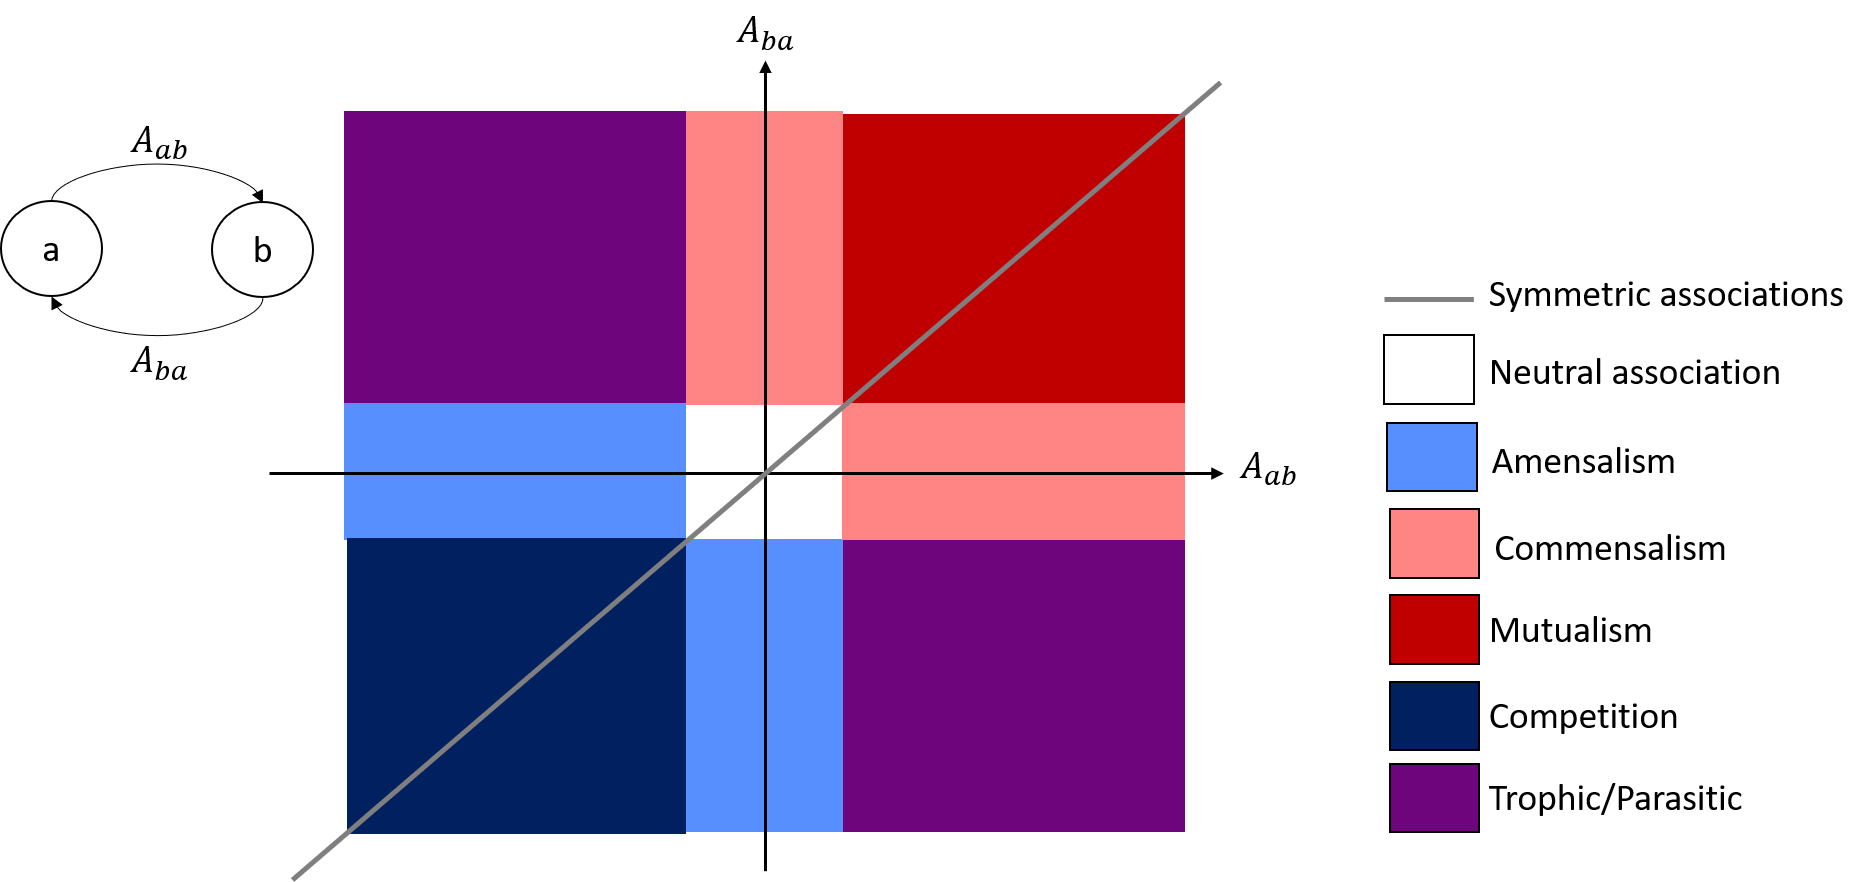
\includegraphics[scale=0.4]{assoc_classif}}
	\caption{Mapping pairwise association strengths to potential interaction classes. The first bissector represents the association domain covered by correlation-based approaches including Joint Species Distribution Models. }
	\label{assocdomain}
\end{figure}

The association strength depends on two latent parameters: the \textit{effect} applied by the source and the \textit{response} of the target. We assume these parameters are controlled by intrinsic traits of the species, which we encode in two separate $d$-dimensional real-valued vectors referred to as embeddings.
In practice, $d$ is a user defined parameter which is typically significantly smaller than half the number of species.

The \emph{effect embedding} of species $\spc$ is denoted as $\rho_\spc$, it captures the type of organisms the species allows when it is present. The \emph{response embedding} of species $\spc$ is denoted as $\alpha_\spc$, it controls the type of biotic context the species would strive in. For instance, trees with spreading canopy create shade (effect) that selects only shade-tolerant (response) species and exclude others.  
The response and effect embeddings of the different species can be collected into two $m\times d$ matices, respectively denoted as $\ResMat$ and $\EffMat$.
The association matrix is then written as
\begin{equation*}
	\AssMat = \ResMat\EffMat^{T}
\end{equation*}

\begin{figure}[h]
	\centering
	\commG{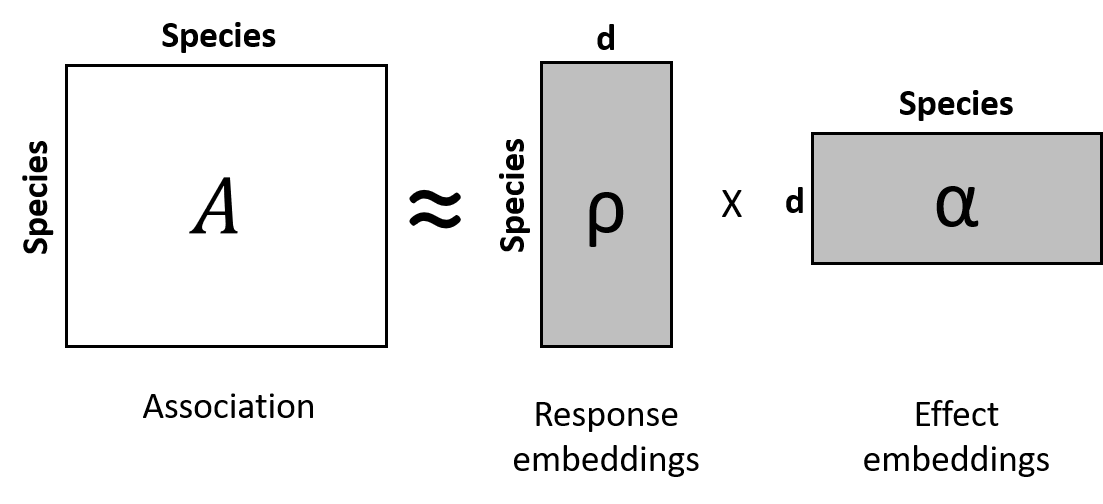
\includegraphics[scale=0.5]{factorization}}
	\caption{Association matrix factorization.}
	\label{factoriz}
\end{figure}

Note that species with similar response embeddings constitute clusters of rows in the association matrix, called \emph{response groups}. Conversely, species with similar effect embeddings consititute clusters of columns in the association matrix, called \textit{effect groups}.
In the network defined by adjacency matrix $\AssMat$, the product of both types of groups, results in the emergence of clusters that can be seen as \emph{structural roles}. 

\subsubsection{Biotic context}
The biotic context encodes our assumptions about potential biotic effects a target species is exposed to in a given site. In the simplest case, without any prior knowledge, it is formed of individuals from other species observed in the same location. Specifically, the biotic context of species $\spc$ in site $\site$, denoted $\BioCont_{\site\spc}$, is computed as follow:
\begin{equation*}
\BioCont_{\site\spc} = \{\ospc \in [1,m], \ospc \neq \spc ~\text{and}~ \abdv_{\site\spc} > 0 \}
\end{equation*}

We obtain the aggregated effect of the biotic context by averaging the effect embeddings of its elements weighted by their respective abundances:   
\begin{equation*}
\BioEff_{\site\spc} = \frac{1}{\abs{\BioCont_{\site\spc}}} \sum_{\ospc \in \BioCont_{\site\spc}} \abdv_{\site\ospc} \cdot \alpha_{\ospc}
\end{equation*}

This formulation allows the compensation between the presence of facilitators and competitors. By weighting with abundance, we consider implicitely that individuals from the same spacies are similar and contribute equally to the community structure. Conversely, the effect of rare species would only be apparent if their per capita effect is stronger than the aggregated effect of dominant groups.

The biotic context carries implicit constraints on the structure of species association networks by restricting the set of potential associations a priori. We present some alternative definitions of the biotic context with the associated data requirements and relevant effect aggregation functions in the appendix~(see Section~\ref{sec:alt-bio}). 


\subsection{A conditional generative model of abundance}

\subsubsection{Formalization}
The indicator of abiotic suitability for species $\spc$ at site $\site$, denoted $\ssuit_{\site\spc}$, follows a Bernoulli distribution, whose parameter (success rate) is given by a habitat suitability model, $\habs$, fitted on the target species's occurrences.
\begin{equation*}
    \ssuit_{\site\spc} \sim \mathcal{B}(\habs_{\spc}(\abiov_{\site}))
\end{equation*}

\begin{figure}[h]
	\centering
	\commG{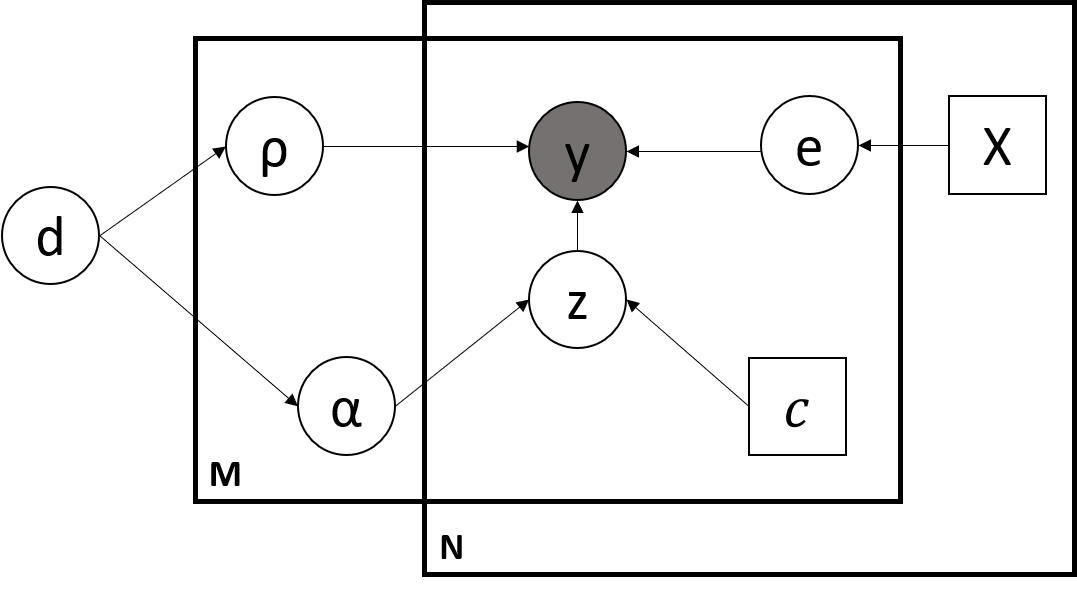
\includegraphics[scale=0.5]{plate}}
	\caption{Plate diagram of the generative model of abundance.}
	\label{plate}
\end{figure}

At sites where the abiotic environment is not suitable (i.e.\ where $\ssuit_{\site\spc} = 0$), the probability mass of the species abundance is concentrated on zero. In other words, $\eta_{\site\spc}$ follows the Dirac delta function denoted as $\delta_0$.

Otherwise (i.e.\ where $\ssuit_{\site\spc} = 1$), the abundance of the species is a function of its biotic context. 
Following (Rudolph et al.\ 2016), we model the abundance using the canonical form of the exponential family $\mathcal{E}$ parameterized by $\eta_{\site\spc}$.
\begin{equation*}
\abdv_{\site\spc} \sim \left\{
\begin{array}{ll}
\mathcal{E}(\eta_{\site\spc}) & \mbox{if } \ssuit_{\site\spc}=1, \\
\delta_0 & \mbox{otherwise.}\\
\end{array}
\right. \\
\end{equation*}

We let the canonical parameter $\eta_{\site\spc}$ depend on the response $\rho_\spc$ of the target species and the biotic context effect $\BioEff_{\site\spc}$. An offset $o_{\spc}$ is used to represent the baseline abundance for each species in the event of an empty biotic context. Link function $\linkf$ scales the outcome to the domain of the target variable. 
%When the offset is set to zero, the target species would need a facilitator to be present. %
\begin{equation*}
  \eta_{\site\spc} = \linkf(\rho_\spc \BioEff_{\site\spc} + o_\spc)
\end{equation*}
which can be rewriten as an aggregate of pairwise association strengths
\mynote{Are the indices on $a$ the right way around?}
\begin{equation*}
  \eta_{\site\spc} = \linkf\big( \sum_{\ospc \in \BioCont_{\site\spc}} \abdv_{\site\spc} \cdot a_{\spc\ospc} + o_j\big)
\end{equation*}

Different choices of probability distributions, depending in particular on the type of data considered (presence/absence vs. abundance) result in different instanciations of this generic model.
In Table \ref{paramap}, we provide the expression of the canonical parameter, the sufficient statistic and the likelihood in the special cases where $\mathcal{E}$ is a binomial (with fixed number of trials), a negative binomial (with fixed number of failures) or a Poisson distribution. 
\mynote{Explain more, which distribution for which scenario, make the columns of the table match the text. What does $\sigma$ stand for?}

%TABLE HERE% 
\begin{table}[bthp]
\begin{tabularx}{1\textwidth} {|s|s|b|}
	\hline
	\textbf{Distribution} & \textbf{Link function} & \textbf{\textbf{Parameter mapping}}  \\
	\hline
	\hline
	Bernoulli  & Identity  & $p_{i,j}=\sigma(\sum_{k \in c_{i,j}} y_{i,k} \mathcal{A}_{j,k} + o_j)$  \\
	\hline
	Poisson  & Identity  & $\lambda_{i,j}=\exp(\sum_{k \in c_{i,j}} y_{i,k} \mathcal{A}_{j,k} + o_j)$  \\
	\hline
	Poisson  & $\log$  & $\lambda_{i,j}=\sum_{k \in c_{i,j}} y_{i,k} \mathcal{A}_{j,k} + o_j$  \\
	\hline
	Neg binomial  & Identity  & $p_{i,j}=\exp(\sum_{k \in c_{i,j}} y_{i,k} \mathcal{A}_{j,k} + o_j)$  \\
    \hline		
\end{tabularx}
\caption{Parameter mapping and link function choices for common distributions}\label{paramap}
\end{table}

\subsubsection{Inference}
We consider a dataset of observed abundances $\abdM$ and environment features $\abioM$ given as input.
We compute the sets of positive (present species) and negative (absent species) examples on each site $\site$:
\begin{align*}
\mathcal{S}_{\site}^+ &= \{\spc \in [1,m], \abdv_{\site\spc}>0\} \\ 
\mathcal{S}_{\site}^- &= \{\spc \in [1,m], \abdv_{\site\spc}=0\}
\end{align*}
Negative examples are typically overrepresented in the dataset, leading to a high inbalance between positive and negative examples. Therefore, we sub-sample negative examples, selecting $r \%$ of them at random into the training set, alongside all positive examples. By introducing noisiness into the objective function, this sub-sampling procedure also improves the robustness of the estimations and prevents overfitting. Furthermore, we promote the sparsity of the embeddings and of the resulting association matrices by adding lasso penalties on the embedding vectors. 
Our model is then trained on this collection of labelled examples. Specifically, we maximize the log-likelihood \mynote{you minimize the negative log-likelihood, hence maximized the likelihood, right?} of the observed abundances on each site for all positive examples. \mynote{what about negative examples?}

In summary, given input data (abundances $\abdM$ and abiotic variables $\abioM$) together with user-defined hyperparameters (including embedding dimension $d$, vector of species offsets $O$ and negative examples subsample rate $r$) the model training procedure aims to infer the value of the model parameters (esp.\ the response and effect embeddings matrices $\ResMat$ and $\EffMat$) that minimize the objective function. To do so, we use online stochastic gradient descent. Details of the objective function and its derivative with respect to each parameter are provided in the supporting material.

% \begin{table}
% \begin{tabular}{|l|l|}
% 	\hline 
% 	Parameters & Hyperparameters \\ 
% 	\hline 
% 	$\Theta=\{\rho,\alpha,\theta_{HSM}\}$ & $\Phi = \{ d, O, \lambda \}$ \\
% 	\hline
% 	$\rho $: response embeddings matrix. & $d$: embedding dimension. \\
% 	$\alpha $: effect embeddings matrix. & $O$: vector of species offsets. \\
% 	$\theta_{HSM} $: Habitat suitability model parameters. & $\lambda$: regularization coefficient. \\
% 	\textbf{ } & $r$: negative subsample rate. \\	
% 	\hline 
% \end{tabular} 
% \caption{Summary of parameters and hyperparameters.}\label{paramlist}
% \end{table}   

\subsection{Validation on simulated data}

Before applying our proposed model on real-world datasets, we perform a validation experiment in a controlled setting. That is, we evaluate the ability of our model to recover interspecific interactions from simulated datasets of known interactions.

\subsubsection{Simulated communities}
We use a process-based stochastic model adapted from \texttt{Virtualcomm} (Gallien and Münkemüller 2015) to simulate the assembly of individuals from a regional species pool into communities, on different locations sampled along an environmental gradient. The assembly process is controlled by three filtering mechanisms: the response to the abiotic environment, the outcome of biotic interactions and reproduction.  For simplicity, the spatial structure of communities and thus dispersal processes are ignored. In other words, there is no exchange of individuals between neighboring communities.

The simulation starts with a given or random initial composition for each community independently. Individuals are replaced through time until an equilibrium state is reached or a user-defined number of iterations is completed. In the end, the final composition of the communities is returned as the result of the simulation.

\mynote{the connection between the paragraphs above and below are not clear to me. Clarify what are the parameters given to the simulation (matrix of interactions, ...), and highlight them below. Did you use random or hand-crafted initial compositions?}

\subsubsection{Experimental setup}
We set up an experiment similar to (Pollock et al, in prep) where multiple simulations are run on 500 random points on a gradient between 0 and 100 with different configurations of the prior interaction matrix. Specifically, four configuration modes were tested: absence of interaction, positive interactions only, negative interactions only and both positive and negative interactions. In each mode, we vary the number of species (5, 10 or 20), the proportion of interacting pairs (sparse, dense) and whether the interaction matrix includes asymmetric effects. Positive (resp.\ negative) effects were all set to $+1$ (resp.\ minus $-1$) as we are interested in the polarity of the interactions rather than their magnitude. The full-factorial design of this experiment produced 29 simulation datasets, summarized in Figure \ref{simexp}).

\begin{figure}[h]
	\centering
	\commG{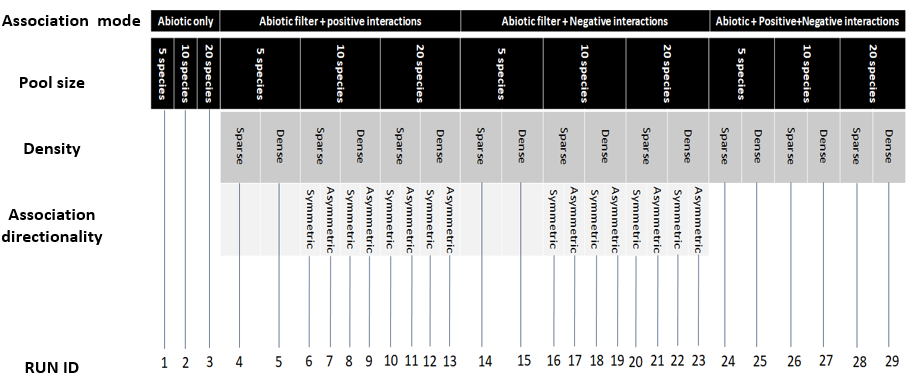
\includegraphics[scale=0.65]{simexp}}
	\caption{Design of the simulation experiment.}
	\label{simexp}
\end{figure} 

\subsubsection{Simulation diagnosis and inference complexity}
As a proxy for the complexity of the inference problem and a simulation diagnosis tool, we evaluate the ambiguity of the patterns of species dependencies present in the simulated communities for the chosen simulation parameters. To do so, for a given pair of source $s$ and target $t$ species, we define two indices that quantify respectively the overlap and the relative variation in abundance of the two species.  

The \textbf{co-occurrence index ($J$)} measures the overlap between the occurrences of the two species.
It is a symmetric index, computed as the Jaccard similarity between the set of occurrences of either species.
\begin{equation*}
J_{st} = J_{ts} = \dfrac{\abs{\{\site \in [n],  \abdv_{\site s} > 0 \text{ and } \abdv_{\site t} > 0\}}}{\abs{\{\site \in [n],  \abdv_{\site s} > 0 \text{ \;or\; } \abdv_{\site t} > 0\}}}
\end{equation*}
Values of $J_{s,t}$ close to $1$ indicate high overlap whereas values close to $0$ indicate near-separation. Values around $0.5$ could indicate average overlap, no conclusion can be drawn. \mynote{I am not sure what average overlap means. The expected overlap also depends on the total number of sites} 

The \textbf{relative abundance increase ($\Delta$)} measures the relative increase in the abundance of the target species when the source species is present. It is an asymmetric measure computed by comparing the abundances of the target species in sites where the source is also present to the average abundance of the target species over all sites where it occurs
\begin{align*}
  \bar{\abdv}_{t} & = \avg(\{ \abdv_{\site,t},  \site \in [n]\text{ s.t.\ }\abdv_{\site,t} >0\}) \\
  \Delta_{st} & = \{ \abdv_{\site,t} - \bar{\abdv}_{t},  \site \in [n]\text{ s.t.\ }\abdv_{\site,t} > 0 \text{ and } \abdv_{\site,s} > 0\} \\
\end{align*}
The larger the standard deviation $\std(\Delta_{s,t})$, the more ambiguous the strength of the effect of species $s$ on species $s$.
If the interval $\avg(E_{s,t}) \pm 1.96 \std(E_{s,t})$ does not contain zero, then the simulated dependencies unambigously translate a polarized effect of species $s$ on species $s$. Otherwise, the polarity of the effect is ambiguous, often due to confounding effects of other species or a neutral association if the mean is close to zero.

\mynote{EG stopped here}
\subsubsection{Training}
For each simulated population dataset, we count the number of individuals of each species in each site to produce a site-by-species abundance matrix and binarize these counts to produce a site-by-species occurrence matrix. 

We model the abiotic response of the species using independent Generalized Linear Models with logistic links and one quadratic term. This model predicts the Habitat Suitability of a location for a target species given its associated environmental value. 

We apply the proposed association inference model with a negative binomial distribution to fit the species counts. We set the offsets for each species as the average value of its abundance on its sites of presence. We also add Lasso penalties with $\lambda=0.01$ on response and effect embeddings to promote the sparsity of their products. 

To select the embeddings' dimension $d$, we use a $5$-fold cross-validation scheme where we monitor the deviance of the predicted abundances. With the selected dimension $d$, we train the model on $1000$ bootstrap samples from the training set and we evaluate its performance on an independent test set using two metrics: Area Under the Curve of the HSM component's predicted probabilities of presence and the deviance of predicted abundances on positive examples. Finally, we compute the $95\%$ confidence interval of the inferred association matrix's mean. 

\subsubsection{Association filtering}
We build the significative association matrix in two steps: statistical filtering and biogeographical filtering. In statistical filtering, we set to zero all associations which confidence interval contains zero and we keep the mean value for the rest. The biogeographical filtering aims to further eliminate associations that could be true given the latent representations of the species. However, they are unlikely to have generated the observed dataset as they are inconsistent with some biogeographical constraints.

For instance, facilitation between two species requires co-existence. Thus, we set to zero any inferred positive effect involving two non-co-occurring species (Sanderson, Pimm et al 2015). On the other hand, competition does not require co-occurrence and may even explain the absence of it. In this case, we assume that negatively associated species should at least live in similar environments for us to consider a potential association. Concretely, we compute the ranges of the environmental values corresponding to their observed points of presence. We retain negative associations among pairs with overlapping environmental ranges or significant similarity (greater than a user-defined threshold) of their habitat suitability parameters, translating akin habitat preferences. 

\subsubsection{Validation metrics}
We formulate an edge classification problem on the fully connected species association network. The problem consists of finding a mapping $f_A$ from any edge (source species, target species) to one of the three effect classes: negative, positive, neutral. Let the pair $(A,\hat{A})$ be composed of the simulated, respectively the inferred, association matrices. We define the true mapping $f_A$ as follow:

\begin{equation*}
\begin{matrix}
f_A : (S_i,S_j) \mapsto  \left\{
\begin{array}{ll}
positive & \mbox{if } A_{i,j}>0, \\
negative & \mbox{if } A_{i,j}<0, \\
neutral & \mbox{otherwise.}
\end{array}
\right.\\\\
\end{matrix}
\end{equation*}

We compute the predicted mapping $f_{\hat{A}}$ similarly using $\hat{A}$ instead of $A$. Finally, we compute the multi-class performance metrics (recall, precision, f1-score) for the predicted classes using the simulation association classes as a reference. (Table \ref{classmet})   

\subsection{Evaluation on empirical data}
In this part, our objective is to evaluate the ability of the model to recover meaningful associations from empirical observations of species abundances. To do that, we use the plant dataset described in (Choler et al.\ 2005). 
\subsubsection{Data description}
The data describes the counts of 84 plant species, collected in July 2000 on 75 units distributed along a mesotopographical gradient. Each unit is of size $5 \times 5 $ m. It is associated to a set of numeric environmental features: the slope inclination in degrees at its location (Slope), the average snowmelt date in julian days between 1997-1999 (Snow), the percentage of non vegetated soil due to physical processes (PhysD) and that due to marmot activity ZoogD. In addition to that, the relative south aspect (Aspect) and the microtopographic landform index (Form) were documented at each location.

\subsubsection{Preprocessing}
We apply a one-hot encoding scheme to the categorical features Aspect and Form and we scale the numerical features. For each plant species, we pretrain an independent generalized linear model with a logit link to predict its occurrences using the preprocessed environmental features as inputs. We use the learnt weights as initial parameter values in the habitat suitability component of our model. 

We define the biotic context for a target species as the set of plants observed on the location of interest. We use a negative binomial distribution to fit the plants' counts jointly as a function of their respective biotic contexts.  We also add an L1 penalty on the embedding vectors' norms to the global likelihood to promote the sparsity of the resulting association matrix. We set the initial value of the embedding vectors using random samples from a uniform distribution on the [-0.01,0.01] interval. Finally, the offset value for each species was set to its average count on occurrence points.

\subsubsection{Training configuration}
We use a multi-label stratified scheme (using the skmultilearn library) to split the observations into training and test sets while ensuring that all species are covered and their proportions are preserved in both sets. 

We proceed to training the full model using Stochastic Gradient Descent (learning rate=0.01, momentum=0.8) on the counts training dataset with a negative examples subsampling rate of $25\%$. We monitor the negative log-likelihood of positive examples (presences) on the validation set after each full pass of the training set to assess the convergence of the training. We stop when the loss stops decreasing or when 200 epochs have elapsed.

\subsubsection{Hyperparameter search and model selection}
For a species pool size $m$, we select the embedding dimension search space on the set of powers of 2 below $m/2$ (to improve hyperparameter search speed). In our case, with $m=82$, values of the embedding dimension K are chosen from the set $\{2,4,8,16,32\}$. 

As we increase the value of the L1 penalty parameter $\lambda$, some components of the embedding vectors take extremely small values for all species (below $\epsilon=10^(-5)$). In this case, these components have no effect on the computed associations. By removing them, the embeddings shrink to a smaller effective dimension $K'$ equal to the number of retained components. Very high values of $\lambda$ lead to $K'=0$, resulting in a zero association matrix. In the latter case, the interaction model is only parameterized by the species offset counts.

For each value of K, we apply the training procedure described previously with increasing values of $\lambda \in \{0.01,0.015,0.02,0.025\}$. We evaluate the resulting models on the test set by computing the effective dimension $K'$ and the deviance of the predicted counts on positive examples. We summarize the model selection results in Figure \ref{gridaravo}.

\begin{figure}[H]
	\centering
	\commG{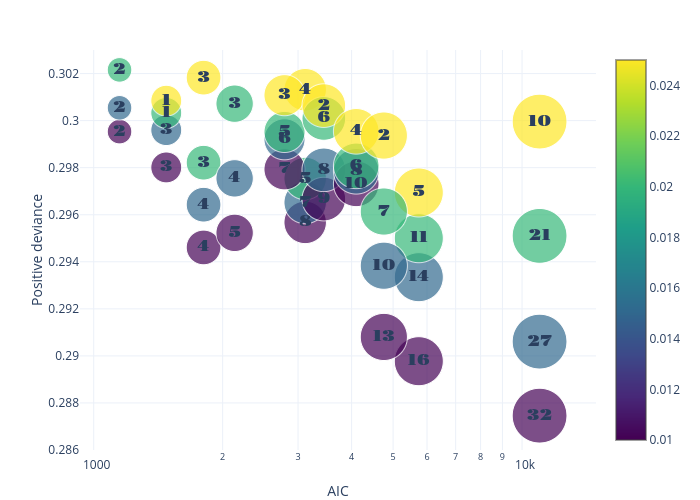
\includegraphics[scale=0.5]{gridaravo}}
	\caption{Positive deviance as a function of the Akaike Information Criterion. Each point represented with a circle indicates a configuration of the hyperparameters. Circle size is proportional to embedding size. Circle color represents the value of the lasso penalty parameter $\lambda$ ranging from 0.01 (darker blueish colors) to 0.03 (brighter yellowish colors). The labels correspond to the number of useful dimensions (non-zero vectors). Larger embeddings lead to a higher model complexity which explains the increasing trend in AIC values with the increase in embedding size. Higher values of $\lambda$ (yellowish points) induce smaller retained dimensions and larger deviance scores. The combination $(\lambda=0.01,K=4)$ provides the best compromise between model complexity and performance.  \url{https://chart-studio.plot.ly/~socco/45}}
	\label{gridaravo}
\end{figure}

\subsubsection{Analyzing plant associations and their latent representations}
In this part, we aim to analyze the inferred associations. We perform a hierarchical clustering on both rows and columns of the association matrix to obtain effect and response groups, displayed in Figure \ref{assocplant:a}. In parallel, we apply the modularity maximization algorithm on the association network to identify densely connected modules, referred to as communities (Gauzens et al 2015). After that, we map the structural roles to the modules to create the group-level network. 

Finally, we investigate the functional determinants of the associations diversity. To do so, we compute the mutual information between the plant traits (Refer to Supplementary materials for full list and documentation) and the learnt representations (Figure \ref{mitraitemb}). The Mutual Information (Shannon and Weaver, 1949; Cover and Thomas, 1991) is an unbounded symmetric and positive score that  measures the amount of information contained in one random variable about another. t quantifies the reduction in uncertainty about one random variable given knowledge of another. Zero mutual information indicates independence. 

In general, we expect traits related to dispersal capabilities (seed, spread) to affect the prevalence of the species, consequently increasing or decreasing the opportunity to affect other species (interaction probability). As a result, they should be important in the structure of effect embeddings. Conversely, traits related to nutrient uptake and biomass accumulation showcase the competitive or cooperative abilities of the plant species. Hence, we would expect a strong influence on both plants' responses and effects.   

\section{Results}
\subsection{Recovering simulated association types}
\subsubsection{Association classification performances}
In average, recall did not vary significantly between positive and negative associations. However, precision was better for the latter. Higher precision was registered for neutral associations. Better performances were reported on smaller datasets with higher recall  on dense association configurations against better precision on sparse configurations. Low precision was registered for positive and negative associations indicating presence of spurious associations. The worst performance was obtained for the sparse asymmetric positive simulation.  

\begin{table}[H]
\centering
\begin{tabular}{|c|c|c|c|}
	\hline 
	\textbf{Association type} & \textbf{Recall $\%$} & \textbf{Precision $\%$} & \textbf{F1-score $\%$} \\ 
	\hline 
	Neutral & $60.75$ & $98.64$ & $74.5$ \\ 
	\hline 
	Negative & $72 $ & $34.02$ & $41.23$ \\ 
	\hline 
	Positive & $77.6$ & $17.6$ & $26.72$ \\ 
	\hline 
	Macro-averages & $62.45$ & $94.71$ & $73.09$ \\ 
	\hline 
\end{tabular} 
\caption{Association classification performances.}\label{classmet}
\end{table}

\begin{figure}[H]
	\commG{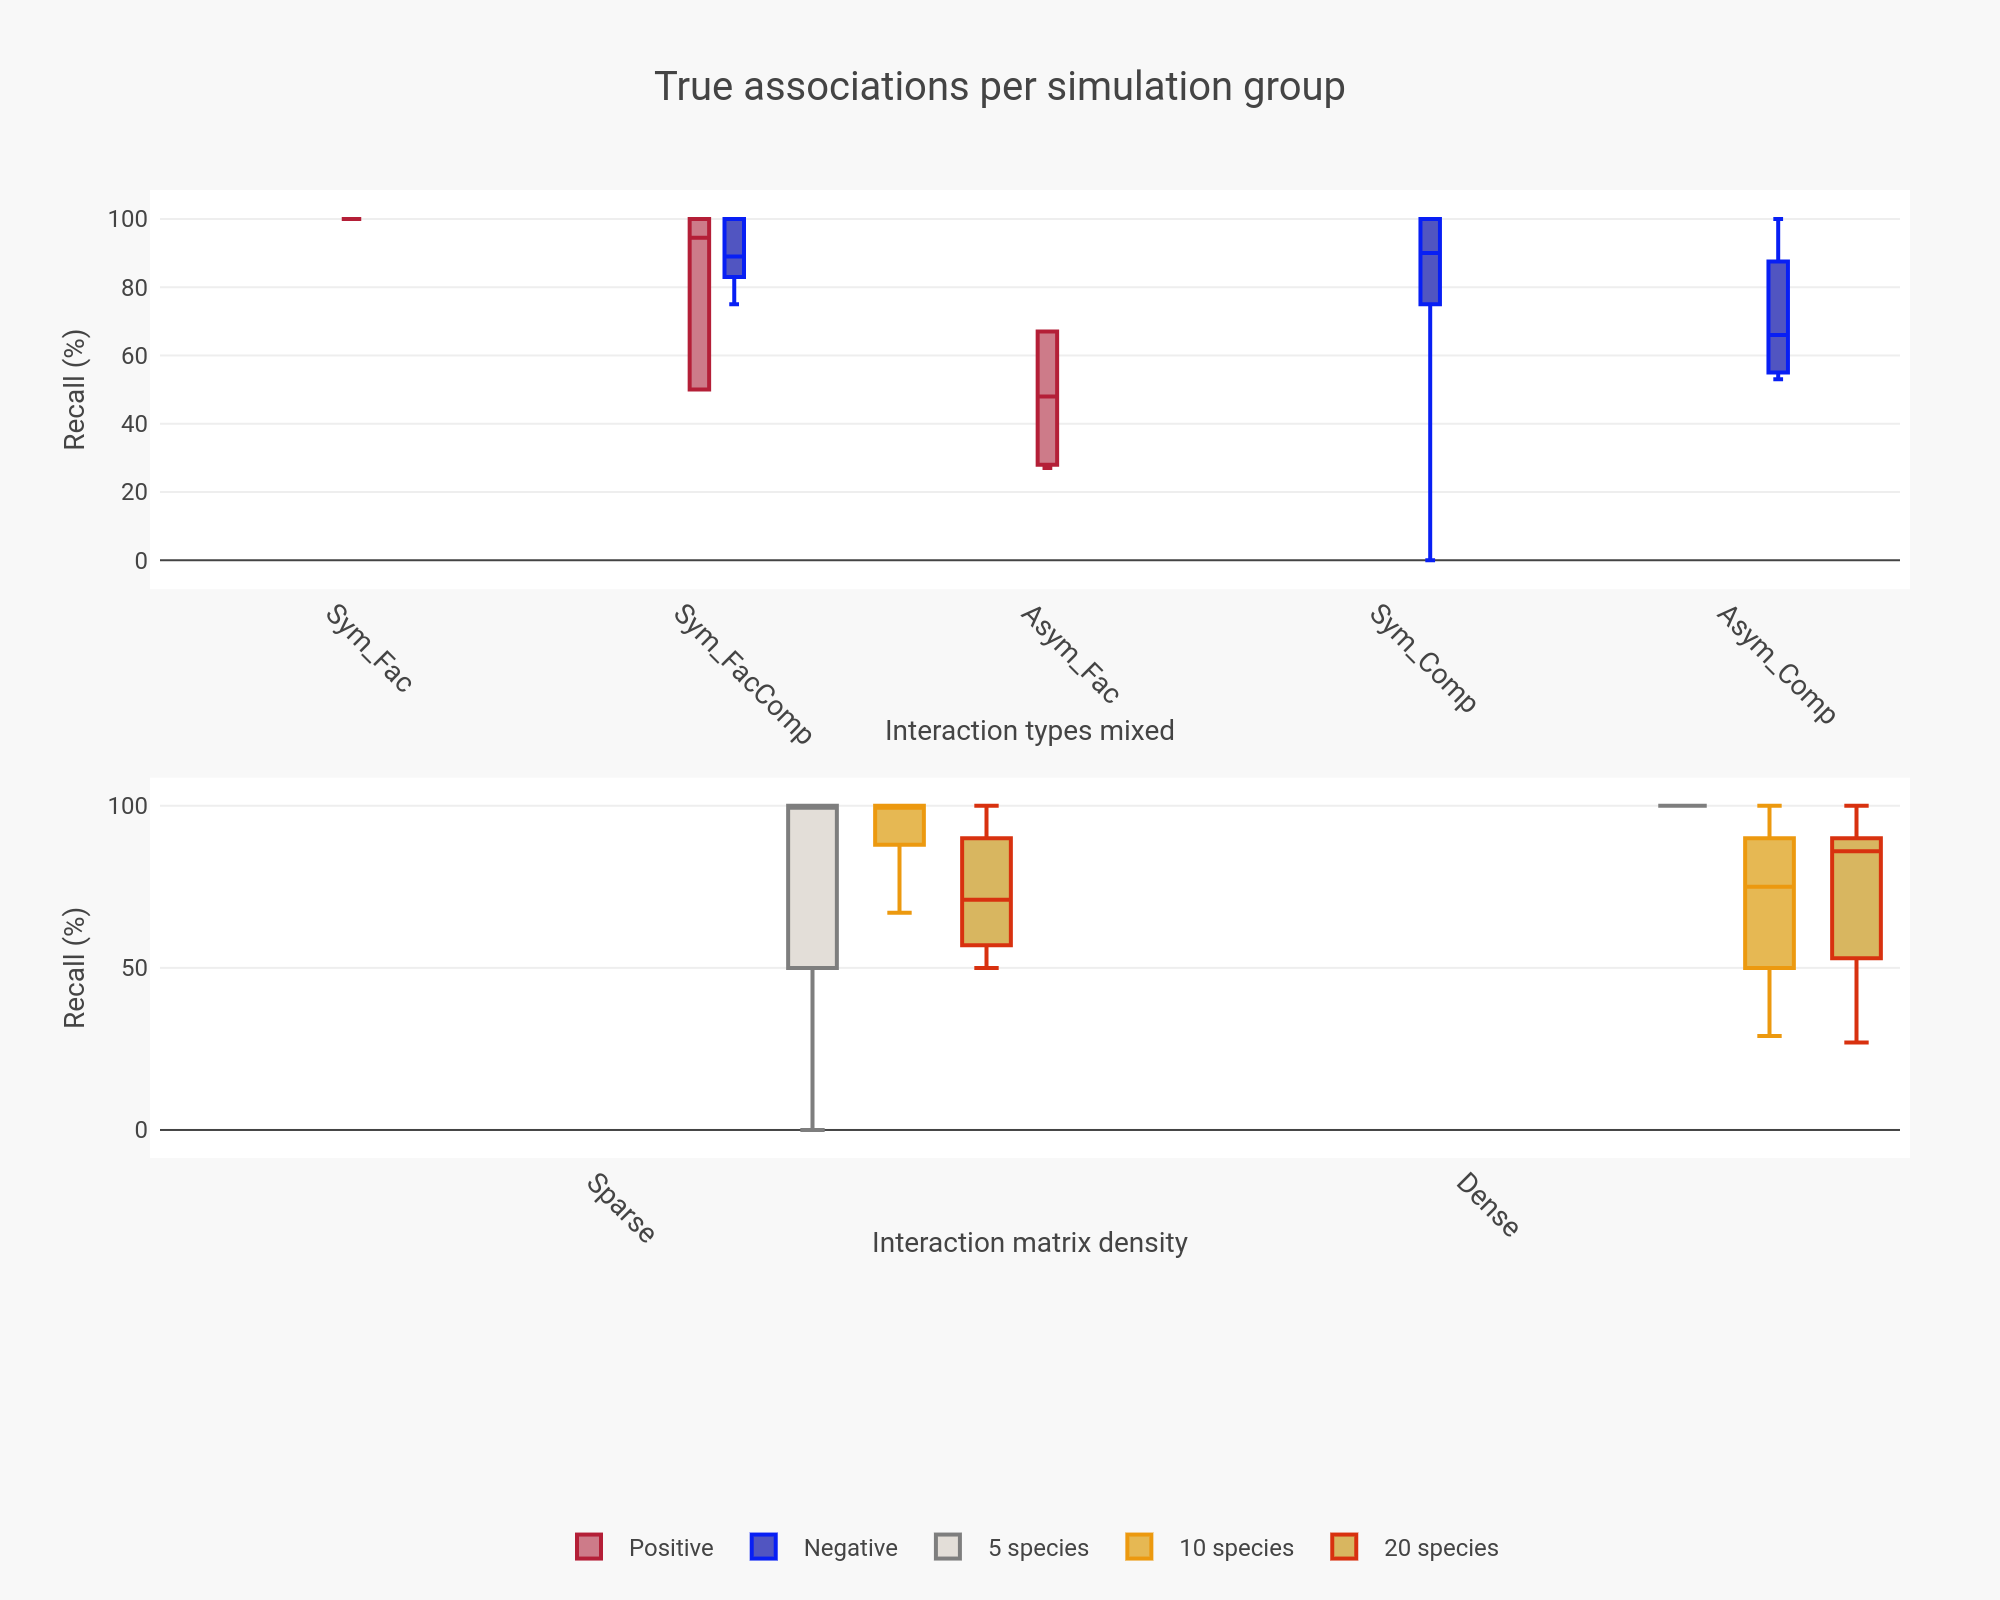
\includegraphics[scale=0.155]{sim_perf}}
	\caption{Recall values per simulation groups. \url{https://chart-studio.plot.ly/~socco/53}}
	\label{simperf}
\end{figure}

On the other hand, biogeographical filtering increases the recall on neutral associations(more correctly identified non interactions) and the precision of positive and negative associations (less spurious interactions).

\subsubsection{Confronting inferred associations to observed patterns}
We find that the observed patterns told different stories about the actual associations. The co-occurrence index was higher than $50\%$ for all species with at least one positive effect. However, the species pairs involved in negative associations appeared together more than expected under the independence assumption in some runs and less on others, in particular on bigger pools. Neutral associations induced co-occurrence indices spanning a large spectrum below $70\%$. 

The Geographic Relative Effect on Abundance index (GREA) reflected well the simulated associations with negative (resp. positive) effects below or around (resp. above) zero, while neutral associations were centered around zero. However, most positive effects yielded small values of their respective GREA indices as compared to the negative effects. Although more clearly marked, the latter approached neutrality on bigger and more densely connected communities. \\ 

\begin{figure}[h]
	\centering
	\commG{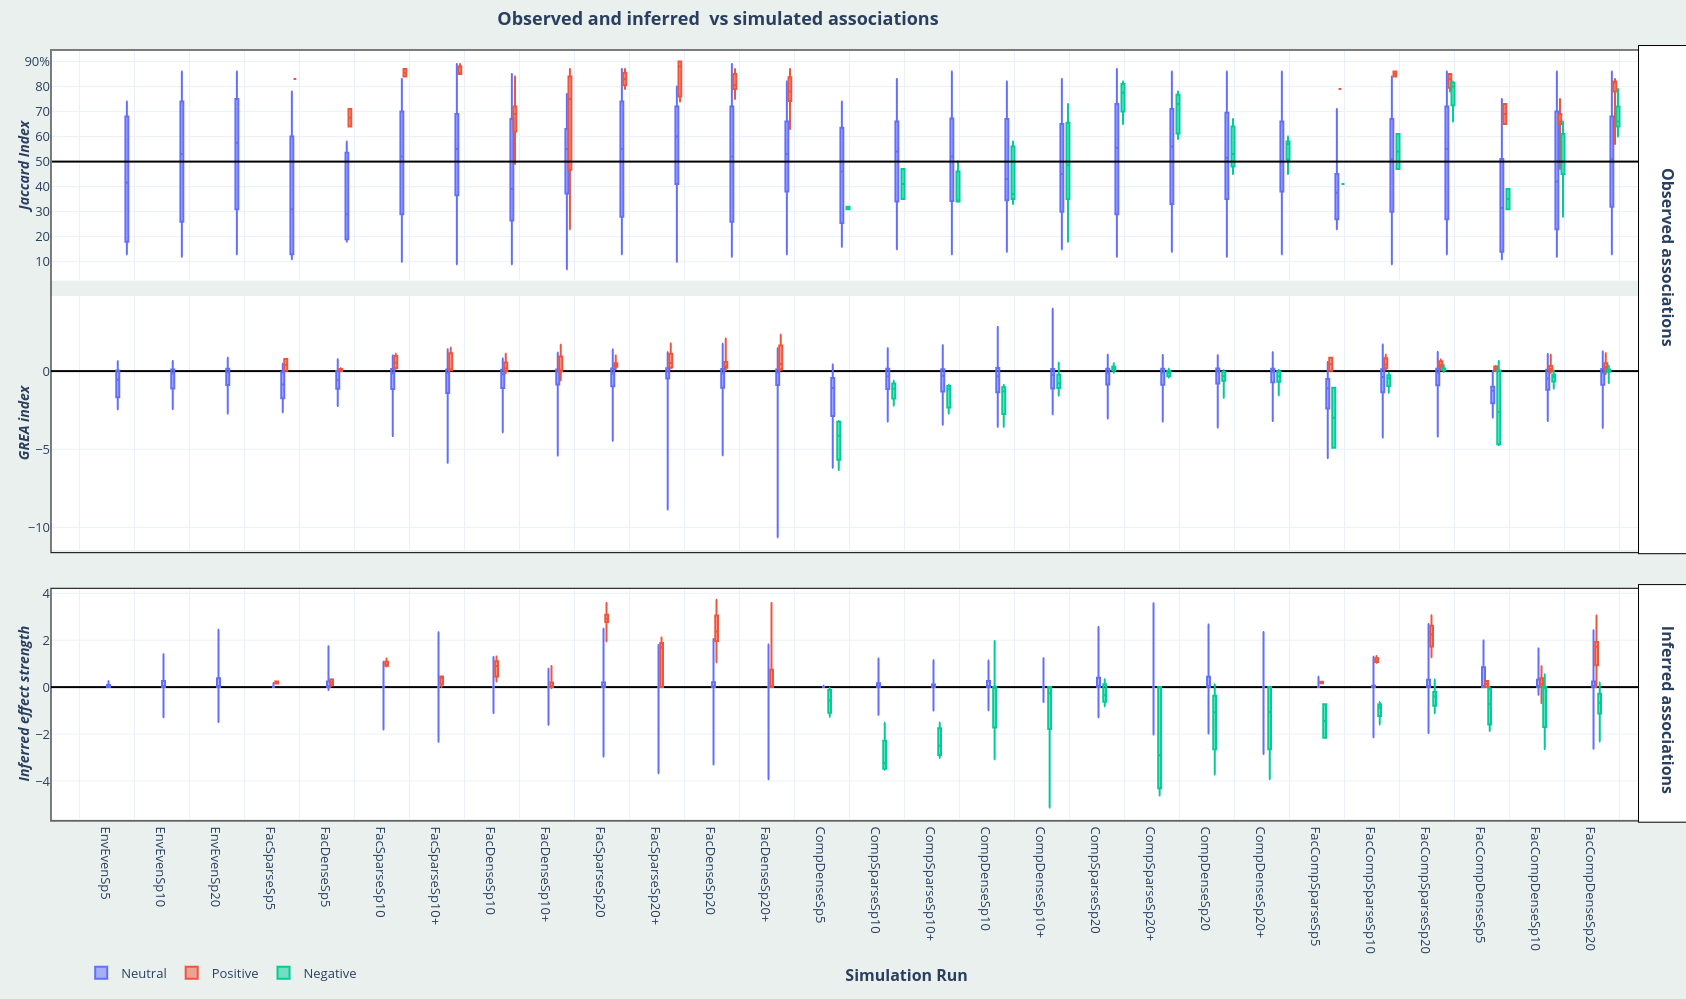
\includegraphics[scale=0.25]{patt}}
	\caption{Distribution of co-occurrence, relative abundance effect and inferred association strength per type of association. \url{https://chart-studio.plot.ly/~socco/30}{Interactive mode}}
	\label{patterns}
\end{figure}

The inference model was able to discriminate positive from negative effects while maintaining an average value for non interacting pairs centered on zero. On simulations with a dense mix of positive and negative associations, both observed effects and inferred associations were close to zero, possibly due to opposite effects canceling each other. 

\subsection{Abiotic and biotic drivers of Alpine plant distributions}
\subsubsection{Plant habitat suitability}
We analyze the parameters and performances of the HSM fitted on plant occurrences. Results are summarized by plant genus groups in Figure \ref{hsmaravo}. The model predicts habitat suitability with at least $70\%$ AUC score for all genuses. The analysis of environmental variable importance shows the dominance of Snow duration followed by zoogenic disturbances, the site form and aspect. Physical disturbance and slope weights were neglectible, probably due to their correlation with Snow. 

\begin{figure}[H]
	\centering
	\commG{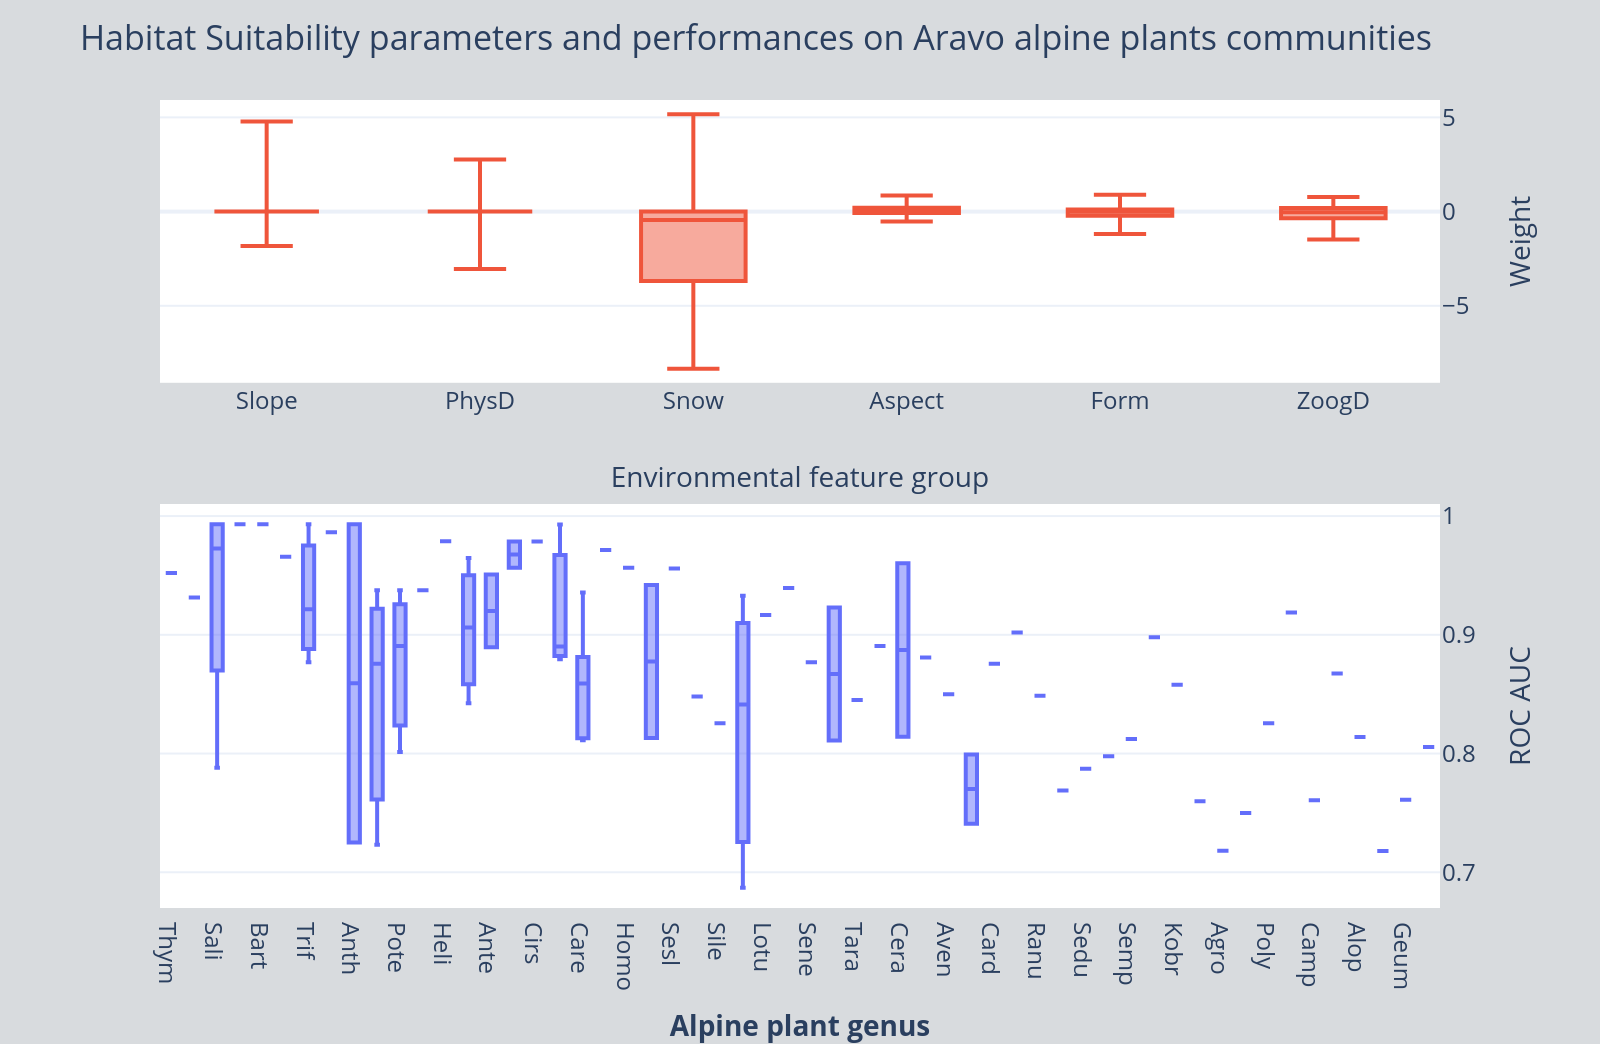
\includegraphics[scale=0.22]{hsmaravo}}
	\caption{Habitat Suitability Model parameter interpretability and prediction performances.\url{https://chart-studio.plot.ly/~socco/1/}}
	\label{hsmaravo}
\end{figure}

\subsubsection{Plant associations on a mesotopographic gradient}
We analyze the inferred associations and the overall network structure (Figure \ref{assocplant}) in light of existing literature on alpine plants interactions (Choler et al 2001). Four densely connected modules stand out. They are structured along the mesotopographical gradient. 
\begin{enumerate}
	\item High-altitude, dry and windy communities densely connected by positive associations: (i) unselective commensalism of forbs by dominant graminoids, (ii) facilitation between graminoids and tall herbs. The latter act as hubs connecting the high elevation sites to the adjacent sites. 
	\item Mid-gradient communities composed of two groups: (i) Tall herb grasslands occuring in favorables conditions, mostly structured by negative associations (ammensalism and competition); (ii) Short herb meadows, prone to zoogenic disturbance. They present higher abundances when co-occuring with tall herbs. Through their spreadth they also play a central role in connecting extreme and favorable sites' communities. 
	\item Chinopholous (cold-resistant) vegetation appearing on late-melting sites. They cohabitate positively with some short-herbs but are negatively affected by forbs and tall herbs. 
	\item North-facing isolated communities dominated by Salix Herbacea negatively associated with high-altitude communities and characterized by high eccentricity.
\end{enumerate}

Modules identified on the basis of link density by the modularity maximization algorithm are spatially structured. Hence, the network of modules reflect the spatial connectivity and as a result the turnover over the gradient. Within each commmunity, we identify various subgroups based on different responses (incoming edges) or effects (outgoing edges) to other groups. 

For instance, the high-elevation module (pink nodes) comprises three subgroups with different structural roles. Graminoids dominate these communities, they provide wind protection to forbs and some tall herbs (Festucal Violacea, Trifolium Alpinum). The latter also occur on grasslands where they compete with each other. Hence, this subgroup is separated from other forbs despite their cohabitation and the similar response to graminoids. 

As reported in the literature (Callaway 2001, Choler 2005), the abiotic stressors strongly structure the distribution of the plant species and the dominant interaction types. Indeed, more positive associations are reported in stressful conditions (high-elevation and late-melting sites). Particularly, the average snow duration seems to be the major structuring force. 
     

\begin{figure}[h]
	\begin{subfigure}{\textwidth}
		\commG{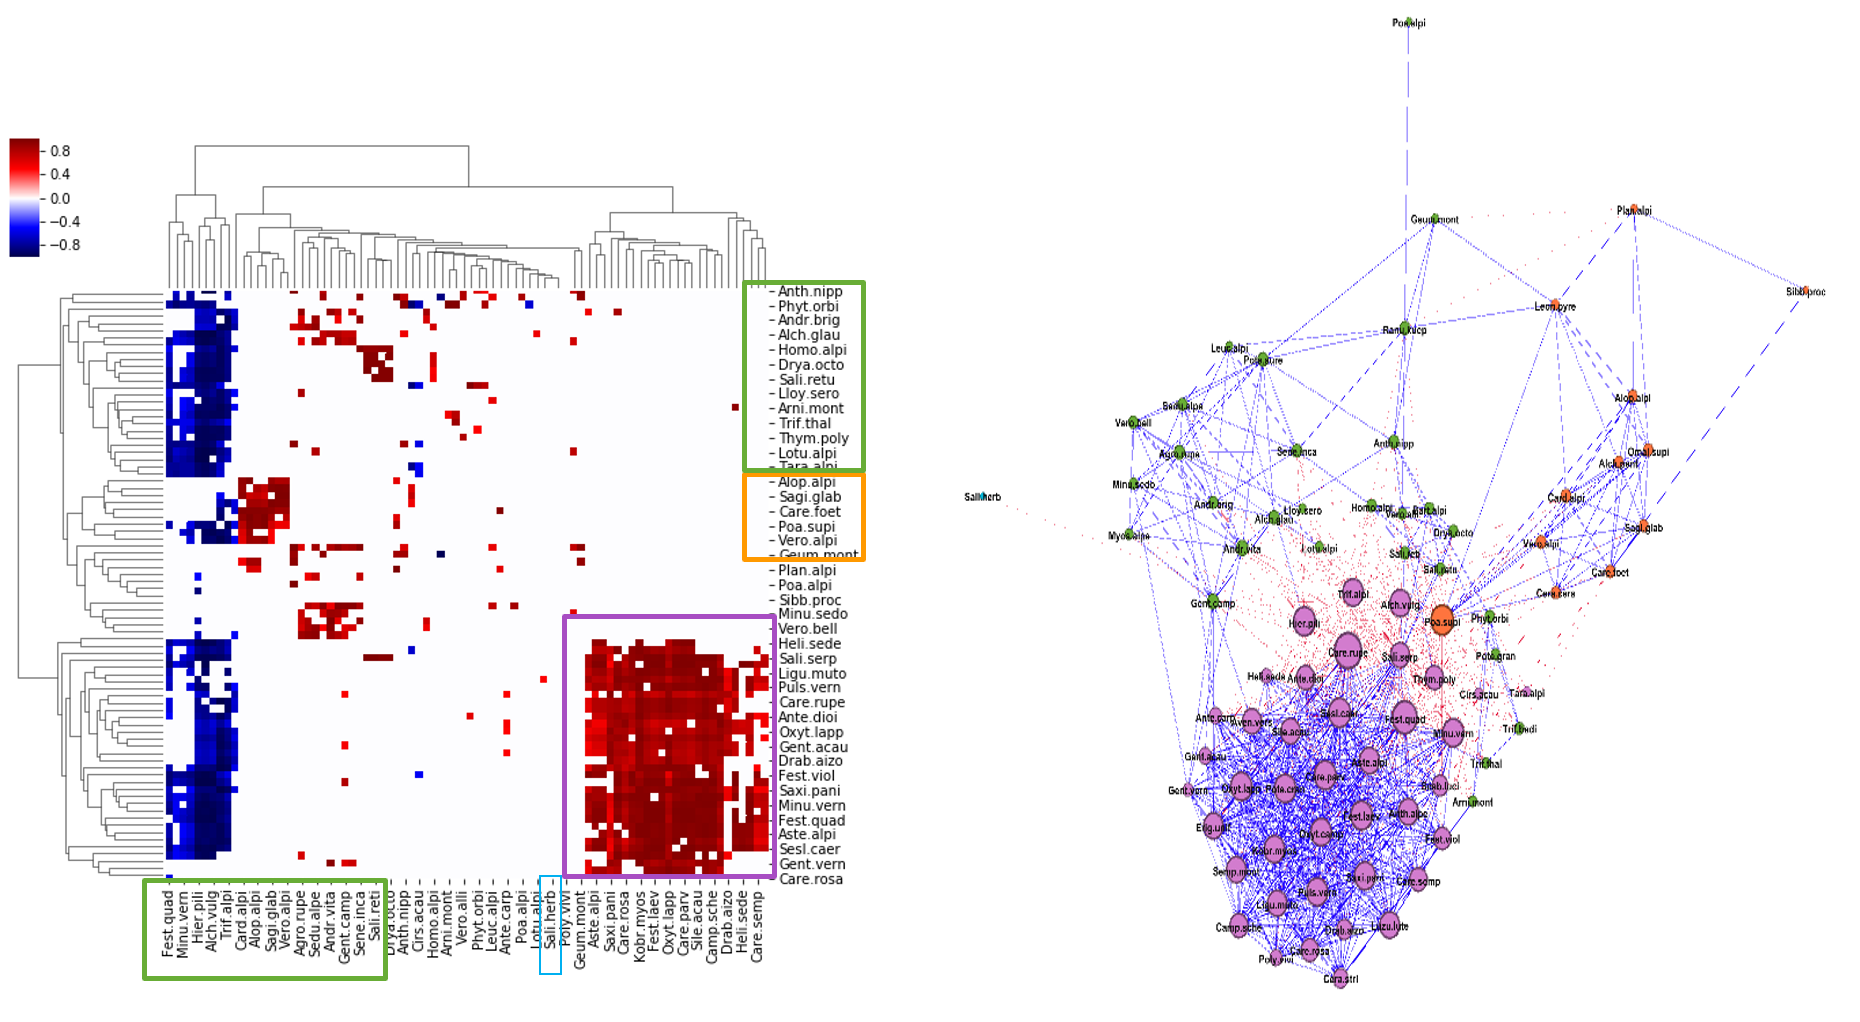
\includegraphics[scale=0.4]{aravoassoc}}
		\caption{Inferred plant association network. } \label{assocplant:a}
	\end{subfigure}
	\newline
	\begin{subfigure}{\textwidth}
		\commG{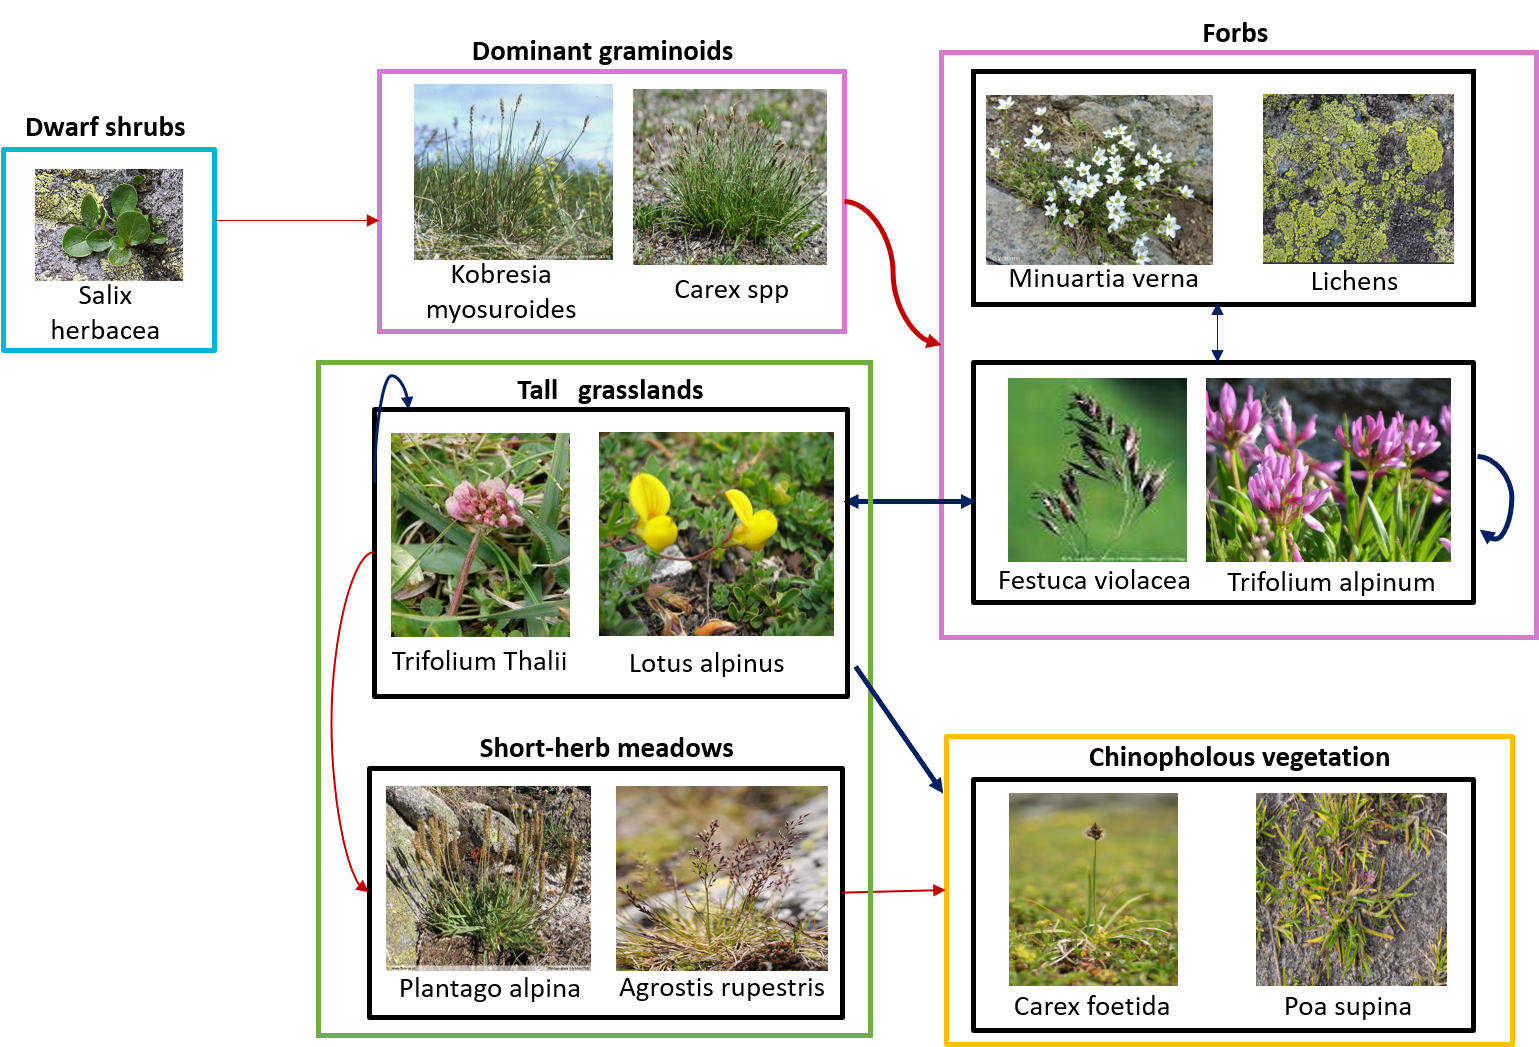
\includegraphics[scale=0.4]{groups}}
		\caption{Summary network of plant associations.} \label{assocplant:b}
	\end{subfigure}
	\caption{Plant associations on an alpine mesotopographic gradient. Subfigure (a) shows the normalized pairwise associations on the left and the corresponding network on the right. Blue (resp. red) edges indicate negative (resp. positive) edge weights. Node colors on the graph represent communities identified by the modularity maximization algorithm (Newman et al 2006). We highlight the communities composition using colored squares on the matrix on the right. Species in the association matrix are grouped based on a hierarchical clusterings performed rowise (yielding response groups) and columnwise (yielding effect groups). Subfigure (b) summarizes the association network at the level of previously identified groups. Edge thickness is proportional to the number of links between the interacting group pair.} \label{assocplant}
\end{figure}


\subsubsection{Functional meaning of plant embeddings}
We analyze in Figure \ref{mitraitemb} the mutual information of learnt latent representations and plant functional traits. The result show a relatively significant contribution of the Nitrogen mass and Spread to the plants response, whereas the angle was found independent. The Specific Leaf Area contributes significantly to the effect in addition to the Nitrogen mass and on a lesser extent height, spread and seed. \\  

\begin{figure}[h]
	\commG{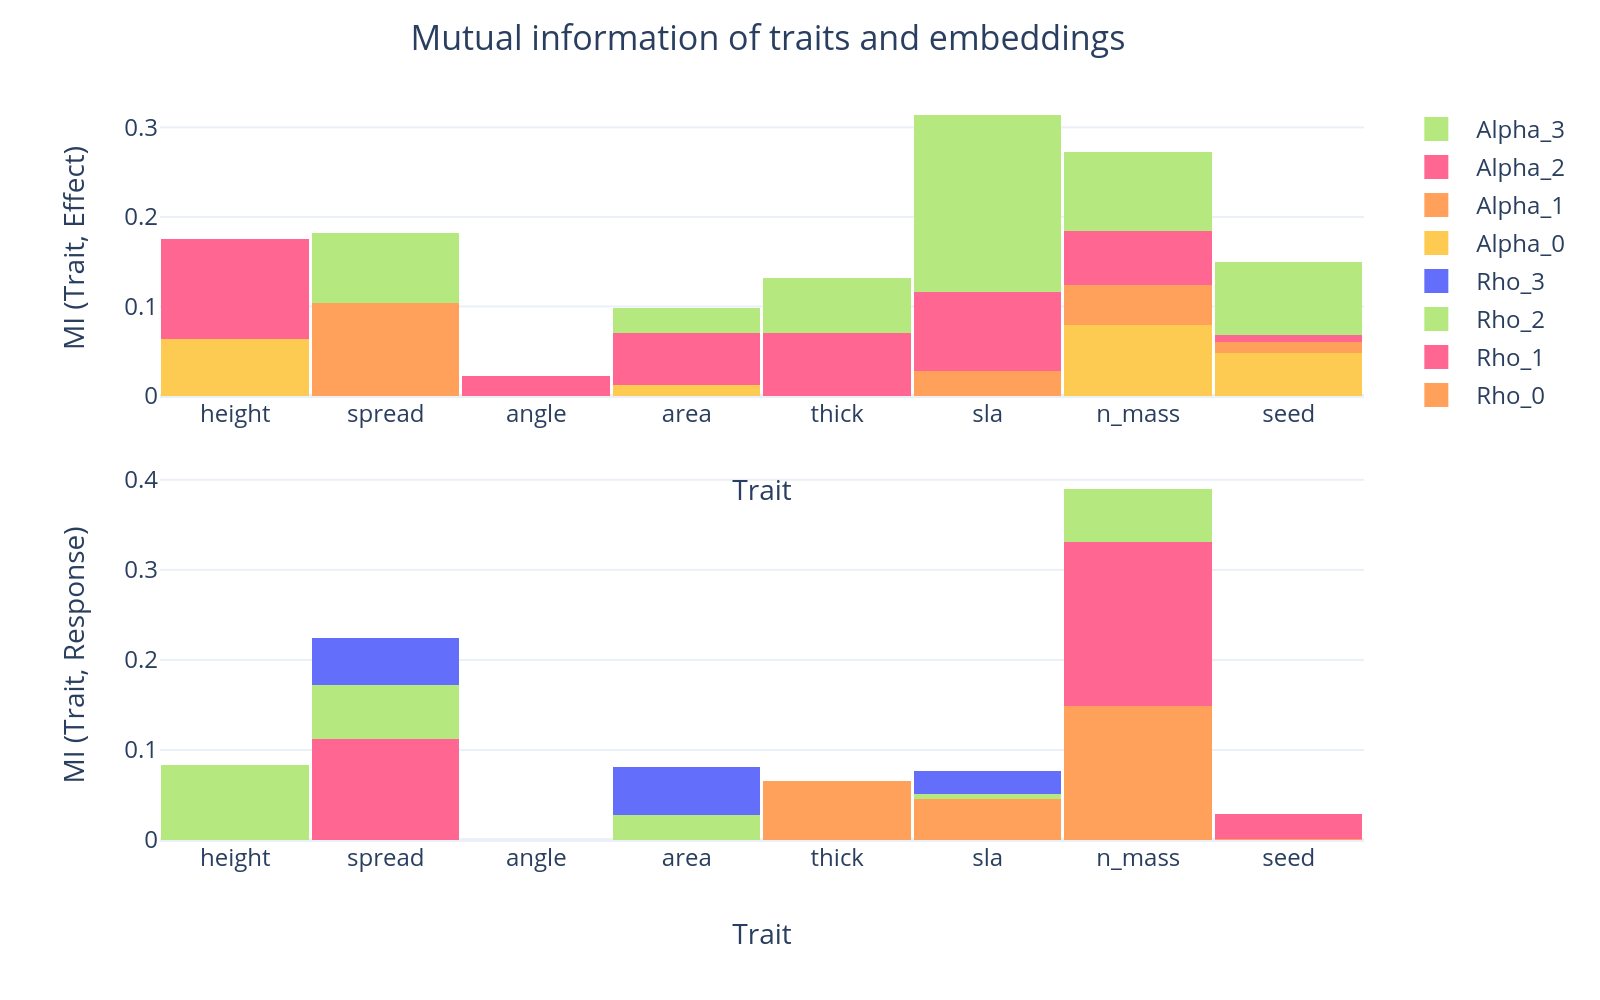
\includegraphics[scale=0.25]{mi_trait_embeddings}}
	\caption{Mutual information between plant traits and their latent representations. Each bar concerns a specific trait, it represents the stack of mutual information scores from the first to the last (fourth) embedding dimension. The lower (resp. upper) figure shows the results for the response (resp. effect) embeddings. \url{https://chart-studio.plot.ly/~socco/70}} \label{mitraitemb}
\end{figure}

\section{Discussion}
%Qu'est-ce qu'on propose ?%
We first develop a probabilistic model of multispecies abundances that accounts for habitat suitability as well as biotic associations. We parameterize this model with an asymmetric association matrix computed from two sets of low-dimensional embeddings representing: the effect present species have on others' abundance, and the response to other species' effects. We then use the model to infer associations given species abundances. 

%Rebondir sur les résultats%
We use a process-based simulation model to generate synthetic community datasets. By analyzing the observed co-occurrence and pairwise conditional abundances, we note that co-occurrence levels can be high even on known competing pairs if the species pool is small and the communities' carrying capacity is large. On the other hand, the abundance reflects better the nature of associations as it is lower than average in presence of negative associations and higher with positive associates. Nonetheless, pairwise abundance effects may turn out to be neutral in presence of multiple confounding effects (Boulangeat et al 2012). Consequently, one should model the pairwise associations conditioned on all other species in order to isolate the different opposing influences. For instance, given a triplet A, B, C such that A (resp. C) influences B positively (resp. negatively). If the same strength is applied by A and B we may observe that all pairs are independent, unless we evaluate the association $ A -> B $ conditioned on C and $C -> B$ conditioned on A. In any case, we still need separate observations where we could quantify both associations separately. 

Thereafter, we test the ability of the model to recover simulated associations. We find that the model is able to disentange positive, negative and neutral associations. But, it generates many spurious associations due to high levels of co-occurrence induced by the simulation model. As opposed to Joint Species Distribution Models, our model is able to recover positive associations between species with similar abiotic niches, for two reasons. First, it does not rely on residuals unexplained by the SDM. Instead, it conditions on the habitat suitability for both species hence the probability of them co-occurring would induce a potential for facilitation. Second, the association is evaluated on the basis of abundance variation in presence of the other species. \\ 

Afterwards, we apply the inference model on plants distributed along a mesotopographical gradient in the French Alps. The associations identified by the algorithm conformed to most of the important specific relationships that we expect to find in the upland plant community (Choler 2001), giving us confidence in the novel methods presented here. We observe more positive associations in extreme conditions (dry, windy or frozen) and negative ones in favorable sites, confirming the stress-gradient hypothesis (Callaway et al 2007). We illustrate using the results on Aravo dataset some of the possibilities allowed by the model. For instance, we can use the association matrix to populate a network, study its modular structure through community detection algorithms and analyze the structural roles, including effect and response groups, occupied by species within communities. Such information is useful to evaluate the functional redundancy within communities. Second, we argue that the learnt representations can be related to functional traits of the species, providing the appropriate traits are measured, to identify the functional drivers of network structure. 

It is now agreed upon that inferred associations are not biological interactions. They represent significant spatial colocation or dislocation patterns, that are informative in a predictive rather than causal way (Mils et al 2012). The specific mechanism that led to these patterns may vary from pair to pair, ranging from direct interactions (e.g trophic), to indirect interactions (e.g engineering). 

The problem of inferring associations from co-occurrence is a major part of ecological modeling publications, as much as biomedical and bioinformatics literature. Existing approaches include JSDMs (Ovaskainen et al 2017) which rely on explaining residual correlations by biotic effects but cannot by design model asymmetric associations. Other major state of art methods are based on probabilistic graphical models including Markov Random Fields (Harris et al 2015, Chiquet al 2017) and Bayesian networks (Mils, Trifonova, Aderhold et al 2012). The former yields undirected networks while the latter impose a directed acyclic structure to the network of associations forbiding feedbacks and the modeling of asymetric effects. 

The most challenging part of this task is that it is completely unsupervised, with no prior or guidance on the expected associations or network. Hence, validating the resulting associations is tricky. It is still feasible to evaluate the veracity of the type of associations by using an edge classification scheme and a list of potential interactions as we've shown. However, it is far more difficult to validate the strength of associations especially when working with snapshot data. As many associations would have a strength around zero, it is also valuable to ask whether one should use higher thresholds to decrease the amount of spurious associations and increase model precision and how to select these thresholds ? Moreover, because many processes influence community assembly, multiple scenarios could lead to the same communities making this problem unidentifiable. In this case, we need not one expected list of associations but all the possible ones or a goodness-of-fit measure that accounts for equivalence between different association combinations. 

A possible way to prevent the unidentifiability issue is to include known information on ecological interactions in the model (Cazelles et al 2015). For instance, (Staniczenko et al 2017) use a Bayesian network with a structure defined a priori, and trains its parameters using an SDM to predict species occurrence probabilities. In our case, such constraints can be defined by altering the biotic context definition. One direct way to do it is to consider a customized biotic context for each species composed of the set of its potential interaction partners in a regional metaweb. 

There is now growing evidence that ecological interactions are context-dependent (Poisot et al 2012, Tikhonov et al 2017), we show in appendix B how to infer associations whose strength is modulated by other covariates (e.g: stress, presence of predator, etc.) Recently developed models account for association variability as a function of the environmental context (Tikhonov et al 2017, Clark et al in prep). Despite the new possibilities offered by these developments, the question of how to validate their results still araises itself.

Finally, although the main purpose of the model is to infer species associations, it is also useful to make conditional predictions of abundances. Another possible usage is to perform link prediction on an incomplete network. The idea is to complete the associations involving a target species by leveraging information from similar node species. \\ 
          
 
\section{Conclusion}
Biological interactions and other processes induce spatial patterns of co-occurrence. Our objective is to disentangle these processes and isolate species dependencies. We present a model of species co-abundances as a function of the habitat and biotic associations. We propose an asymetric scheme for modeling associations that is based on learning latent representations of species responses and effects. Future efforts should be directed towards a combination of prior knowledge on the complete or partial topology of the association networks to guide the inference process. Along with that, a strong theory of how known ecological interactions influence the co-distribution of species is needed to support all these models.   

\appendix

\section{Derivatives of the optimized objective}
\label{sec:derivatives}
Canonic derivatives (refer to Liping liu et al 2017). 

\section{Alternative biotic context definitions}
\label{sec:alt-bio}
\subsection{Associations that depend on external factors}
In the base model, the outcome of any pairwise interaction is invariant with respect to the abiotic or biotic conditions surrounding it. To account for that, we introduce a slight alteration to the vanilla model where we allow the embeddings of the biotic context to depend on some chosen variables. We stack the latter in a vector of $p$ covariates noted $V$, such that $V_{ij}$ denotes the value of the $j^{th}$ covariate on the $i^{th}$ site. 

Given an embedding dimension of $d$ latent variables, we start by computing the weight attributed to each dimension as a regression function $g$, with a parameter vector $\gamma$, over the conditioning covariates.      

\begin{equation*}
\begin{matrix}
g: \mathbb{R}^p \mapsto \mathbb{R}^d \\\\
\beta_i=g(V_i ; \gamma)
\end{matrix}
\end{equation*}

For instance, we could set:
\begin{equation*}
\begin{matrix}
g: V \mapsto \gamma \cdot V + 1_d \\
\end{matrix}
\end{equation*}

In which case:  
\begin{equation*}
\begin{matrix}
\beta_i= \sum_{l=1}^{d} \gamma_l \cdot z_{i,l} + 1  \\\\  
\end{matrix}
\end{equation*}

The resulting biotic context can be embedded as follow, where $*$ is the element-wise vector product: 

\begin{equation*}
\begin{matrix}
z_{i,j} = \beta_i * (\frac{1}{|c_{i,j}|}\sum_{k \in c_{i,j}} y_{i,k} \alpha_{k}) = \frac{1}{|c_{i,j}|}\sum_{k \in c_{i,j}} y_{i,k} (\beta_i * \alpha_{k}) \\\\
\end{matrix}
\end{equation*}

\textbf{Recovering the biotic associations}: We proceed similarly to the vanilla model by isolating the pairwise interactions on the response variable. In this case, instead of a 2D matrix, the associations we obtain are retrieved in a three-dimensional tensor $\mathcal{A}$. Each slice on the first dimension of $\mathcal{A}$ represents a local association network.

\begin{equation*}
\begin{matrix}
\mathcal{A}_{i,j,k} = \sum_{l=1}^{d} \beta_{il} \cdot \rho_{jl} \cdot \alpha_{kl} \\\\
\eta_{i,j} = f(\frac{1}{|c_{i,j}|} \sum_{k \in c_{i,j}} y_{i,k} \mathcal{A}_{i,j,k} + o_j)\\\\
\end{matrix}
\end{equation*}

By incorporating the environmental covariates on the latent space, we gain two desirable properties. First, we get a fixed number of parameters that is a factor of the embedding dimension, which is significantly smaller than the number of modeled species. Second, we ensure species with similar latent traits, willingly captured by the response and effect embeddings, share associations regardless of the surrounding conditions. As a result, response or effect groups of species computed from the learnt embeddings remain consistent in the environmental space. 

\subsection{Temporal model}
%Drawback of basic model, causality % 
When time-series are available, we model the target variable $y_{ij}^{(t)}$ denoting the abundance of a species $T_j$, on a location $S_i$, at a certain time $t$. We do that by simply changing the \textbf{biotic context} definition to: \textit{the set of species, including the target, that were observed in the previous timestamp.}

\begin{equation*}
\begin{matrix}
c_{i,j}^{(t)} = \{k  \mid y_{i,k}^{(t-1)}>0 \} \\\\ 
z_{i,j} = \frac{1}{|c_{i,j}^{(t)}|}\sum_{k \in c_{i,j}^{(t)}} y_{i,k}^{(t-1)} \cdot \alpha_{k}\\
\end{matrix}
\end{equation*}
% Graphe dynamique déroulé puis moralisé %

\subsection{Spatial model}
Given a distance measure $\delta$ and a radius $r$, we consider a spatial extension of the model where the \textbf{biotic context} is defined as : \textit{the set of species that were observed at a significatively close location.}

\begin{equation*}
\begin{matrix}
c_{i,j} = \{(s,k)  \mid \delta(S_i,S_s)\leq r \text{ , } y_{s,k}>0 \} \\\\ 
\end{matrix}
\end{equation*}

One can use multiple radius values customized to the dispersal abilities of each target group or species for instance. The effect of each contextual element is subdued by its distance to the target location. The hyperparameter $\tau$ controls the decrease in importance per unit of distance. Similarly, $\tau$ can be customized for each group of species by expert knowledge.  

\begin{equation*}
\begin{matrix}
z_{i,j} = \sum_{(s,k) \in C_{i,j}} y_{s,k} \cdot \alpha_{k} \cdot \exp^{(-\delta(S_i,S_s) \tau)} \\
\end{matrix}
\end{equation*}
%Substituting time for space. 
%space for time substitution, dispersal mechanisms (negative context and competition)

\subsection{Graph biotic context}
So far, we defined the biotic context using the community composition in terms of species and eventually their abundances. At this point, we are able to capture pairwise additive effects. However, we miss the impact of interactions between context species or the whole network structure around the target location on the abundance distribution of the target group. 

Fortunately, graph embedding algorithms permit the incorporation of structured data such as knowledge graphs into predictive models. For instance, we can define the \textbf{biotic context} as the interaction network at the focal point $S_i$ minus the target species $T_j$, noted $\mathcal{G}_{i/j}$. The \textbf{context embedding} is obtained by applying a graph kernel function $\mathcal{K}$ with parameter $\alpha$ on the contextual network.

\begin{equation*}
\begin{matrix}
z_{i,j} = \mathcal{K}(\mathcal{G}_{i/j} ; \alpha) 
\end{matrix}
\end{equation*}


\end{document}

%%% Local Variables:
%%% mode: latex
%%% TeX-master: t
%%% End:
